%% CHAPTER 2 (probably)
%% HCHO Levels

\chapter{TODO: move to biogenic isop chapter: Formaldehyde product over Australia} % Main chapter title
\label{ch_HCHO} %better reference name like ch_HCHO

%----------------------------------------------------------------------------------------
%%	SECTION
%----------------------------------------------------------------------------------------
%TODO: move this one
\section{Australian Biogenic Volatile Organic Compounds (BVOCs)}
  \label{ch_HCHO:sec:bvoc}

  \subsection{Isoprene, Monoterpenes}
    
     
    
    Estimates of isoprene emissions require more work in order to generate confidence at a global scale.
    Due to isoprene being optically thin (see section \ref{ch_HCHO:sec:satelliteHCHO:OpticalDepth}) and having a short life time (around an hour) there are relatively few accurate measurements against which a comparison and verification can be made.
    
    The emissions of isoprene have been modelled at around 500~Tg C yr$^{-1}$ in \citet{Guenther1995} using MEGAN, and more recently around 465~Tg C yr$^{-1}$ in \cite{Messina2016} using ORCHIDEE.
    The global emission factors model used to derive these estimates is based on modelling emissions from different plant species (phenotypes), and very few are used to set the emission factors of Australian forests.
    
    Globally around 710 - 1150 Tg C yr$^{-1}$ of BVOCs are emitted \citep{Guenther1995,Lathiere2006,Guenther2012}.
    90\% of these emissions come from plants and trees, with the most dominant species being isoprene (C$_5$H$_8$) ($\sim50\%$), monoterpenes (C$_10$H$_16$), methanol (CH$_3$OH), ethanol (C$_2$H$_6$O), acetaldehyde (CH$_3$CHO), acetone ((CH$_3$)$_2$CO), ethene (C$_2$H$_4$) and propene (C$_3$H$_6$) (together making up $\sim30\%$) \citep{Guenther2012}.
    The larger of these estimates come from MEGAN, a bottom-up biogenic emissions model which is highly sensitive to several parameters including soil moisture and plant functional type.
    Another model (ORCHIDEE, with inputs similar to MEGAN) estimates $752\pm16$ Tg C yr$^{-1}$, sensitive to terrestrial vegetation variations \citep{Lathiere2006}.
    
    One problem with current estimates of biogenic VOC emissions in Australia is that the emission rates from various species of eucalypt and other flora are highly complex, depending on current and recent weather, temperature, tree age, health, etc. \citep{Guenther2012}. 
    With this complexity added to the diversity of tree species in Australia as well as sparse rural data collections it is hard to model and verify emissions.
    Isoprenoid emissions remain to be verified in Australia and the few monoterpene emission rates we have may be underestimated by a factor of 2-4 \citep{Winters2009}.
  
  \subsection{Biomass Burning}
    As biomass burning can be a large local or transported source of HCHO, CHOCHO, and other precursors to BVOC emissions, it is advantageous to filter out this source.
    One complication when computing HCHO yield from VOC emissions is biomass burning interference, as smoke plumes can carry HCHO and some precursors which.
    Influence from biomass burning can be removed through measurements of acetonitrile and CO (eg: \citep{Wolfe2016, Miller2017}, or else removal of scenes coincident with satellite detected fire counts and aerosol absorption optical depth as done in \cite{Marais2014}.
    \citet{Wolfe2016} disregard HCHO measurements when acetonitrile > 210~pptv and CO > 300~ppbv, while acetonitrile > 200~pptv is used to determine fire influence in \cite{Miller2017}.
    
  \subsection{MEGAN}
    One method used to estimate global isoprene (among other species) emissions is the Model of Emissions of Gases and Aerosols from Nature (MEGAN). 
    MEGAN is a global model with resolution of around 1~km, and is used to generate the BVOC emissions used in various global chemistry models such as GEOS-Chem.
    MEGAN uses leaf area index, global meteorological data, and plant functional types (PFTs) to simulate terrestrial isoprene emissions.
    The various PFTs are used to generate emission factors which represent quantities of a compound released to the atmosphere through an associated activity.
    For example, an emission factor for isoprene within a forest would include the requirement of sunshine and suitable temperature.
    The schematic for MEGAN, taken from \citet{Megan_Website}, is shown in figure \ref{ch_HCHO:fig:megan_schematic}
    
    \begin{figure}[!htbp]
      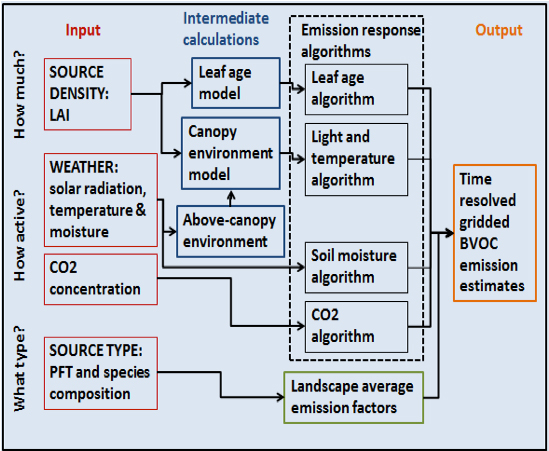
\includegraphics[width=\textwidth]{Figures/MEGANmodel_img.jpg}
      \caption{MEGAN schematic, copied from \citet{Megan_Website}}
      \label{ch_HCHO:fig:megan_schematic}
    \end{figure}

    MEGAN output in Australia is adversely affected by poor emission factor estimation, which is based on plant type classifications (PFTs) and local conditions like soil moisture and weather. 
    An example can be seen in \citet{Muller2008} where MEGAN overestimates isoprene in northern Australia.
    Underestimates of monoterpenes emissions are also seen from MEGAN (TODO: ask Jenny what other paper showed this?), which may be due simply to underestimated emission rates for many Eucalypt species \citep{Winters2009}.
    
    
%----------------------------------------------------------------------------------------
%	SECTION
%----------------------------------------------------------------------------------------  
\section{Satellite HCHO measurements}
\label{ch_HCHO:sec:satelliteHCHO}
  \subsection{Satellite Retrievals}
    Satellites remotely sense atmospheric trace gases through irradiance measurements of solar light which has reflected off the earth's surface. 
    These irradiances are affected by gases which exist along the reflected path of light between the detector, earth, and sun. 
    The irradiance is then used to estimate how much of a particular gas exists along this path, which gives us an estimate which is called a slant column (SC).
    The retrieved SC of a particular gas (or species) can be transformed into a vertical column (VC) by scaling the path length in conjunction with accounting for the trace gas' light scattering properties.
    The scaling coefficient created to transform from SC to VC is called the Air Mass Factor (AMF).

    One satellite is NASA's Earth Observing System's (EOS) Aura, which houses the Ozone Monitoring Instrument (OMI), a near-UV/Visible Charged Coupled Device (CCD) spectrometer.
    Aura orbits the earth in a polar sun-synchronous pattern, circling the earth on a plane coincident with the sun and the poles.
    OMI measurements are used to map several atmospheric trace gases, including NO$_2$, SO$_2$, BrO, HCHO, O$_3$, and aerosols.
    OMI measurements occur from right to left on a band covering 115$^{\circ}$, resulting in swaths of around 2600~km, with pixel sizes from 13x24~km$^2$ at nadir to 26x135~km$^2$ at the swath edges \citep{Abad2015}.
    The swaths cover Earth daily, although half of these are at night time and contain no useful near-UV/Visible information.
    From here on the word pixel is used to describe one data point retrieved by OMI, each pixel includes a latitude and longitude within OMI's data product.
    
    Atmospheric HCHO can be measured using Differential Optical Absorption Spectroscopy (DOAS), as long as trace gases with similar features near the same wavelength are accounted for.
    OMI fits HCHO slant column densities (SCD) along a solar backscatter path within the spectral window of 327.5-356.5~nm \citep{Chance2000}.
    TODO: Go through Lee2005 or Volkamer2005 and detail the DOAS Retrieval of HCHO.
    A DOAS fit determines the total column amount of a trace gas along the path that the instrument views.
    This uses the Beer-Lambert law where radiance is reduced as light travels through a medium.
    The full method details for slant column retrieval by OMI are outlined in section \ref{ch_HCHO:sec:OMI_BOAS}.
    
    Uncertainty in a single pixel for OMI is quite high, roughly the same magnitude as HCHO background levels.
    Figure \ref{ch_HCHO:fig:eightDayUncertainty} shows uncertainty over Australia after one and eight days of averaging at 0.25$^{\circ}$ longitude by 0.3125${\circ}$ latitude.
    There are several methods of calculating this, one of which is used here and compared against the provided uncertainty (TODO) as shown in Section \ref{ch_HCHO:sec:OMIuncertainty}.
    If we assume the uncertainty is random error, and not bias introduced through calculation techniques, then we are able to reduce the uncertainty through averaging.
    Random error can be reduced by either temporal or spatial averaging, decreasing uncertainty by a factor of $1/\sqrt{N}$ where N is the number of observations being averaged.
    High resolution low detection limit estimates can be built up using ``oversampling'', which averages satellite measurements over time.
    A good example can be seen in \cite{Zhu2014} where 0.2$^{\circ}$ by 0.2$^{\circ}$ resolution with high enough sensitivity to see anthropogenic HCHO is acheived with three summers worth of satellite data.
    
    
    \begin{figure}[!htbp]
      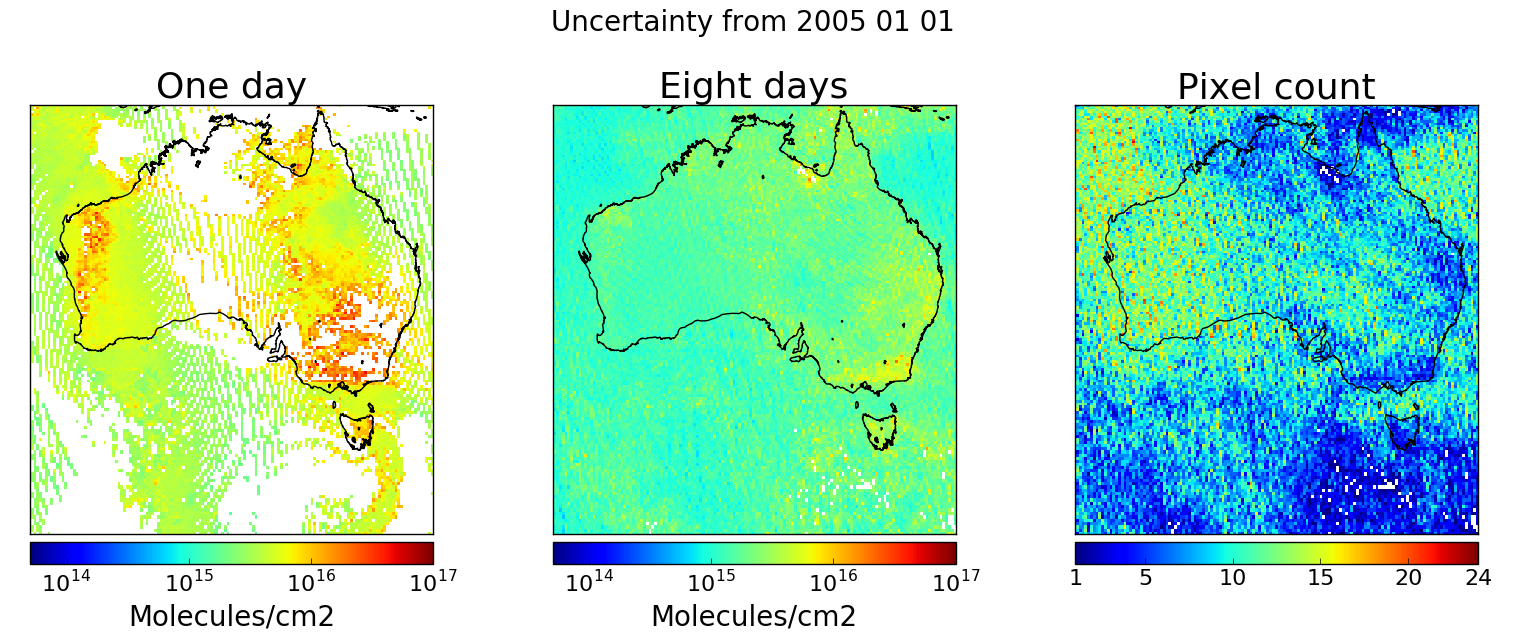
\includegraphics[width=0.7\textwidth]{Figures/HCHO/Uncertainty.png}
      \caption{%
	      OMI uncertainty before and after gridding and averaging 8 days from Jan 1 2005 to Jan 8 2005.
	      The third panel shows the number of pixels in each grid box after 8 days of averaging, before accounting for fire.
      }
      \label{ch_HCHO:fig:eightDayUncertainty}
    \end{figure}
    
  \subsection{OMI Algorithm BOAS}
    \label{ch_HCHO:sec:OMI_BOAS}
    The following information comes from the OMHCHO dataset documentation at \citet{Kurosu2014} and \citet{Chance2002}.
    The method of HCHO total column retrieval depends heavily on measured solar radiation.
    Radiance is directional radiant flux, expressed in Watts per square metre per steradian (a unit of angle used in three dimensional geometry).
    Irradiance is radiant flux received by a surface, expressed in watts per square metre.
    An OMI granule is the sunlit portion of an orbit (one day).
    
    The BOAS algorithm used by OMI is as follows.
    Slant column abundance can be determined by fitting measured radiance (I) at particular wavelengths ($\lambda$), using modelled absorption cross sections ($\sigma$), effective albedo (A) including Rayleigh scattering, a correction for the Ring effect (c$_R\sigma_R$), and a closing polynomial (coefficents c$_0$-c$_3$).
    \begin{equation}
      \label{ch_HCHO:eqn:BOAS_HCHO}
      I(\lambda)  = A I_0 \exp {\left( - \Sigma_i S_i \sigma_i \right) } + c_R\sigma_R + c_0 + c_1(\sigma-\bar{\sigma}) + c_2(\sigma - \bar{\sigma})^2 + c_3(\sigma - \bar{\sigma})^3 
    \end{equation}
    
    For HCHO, absorption cross sections and number densities for interfering gases are determined beforehand.
    This is due to HCHO being so optically thin and interferences must be accounted for precisely \citep{Chance2002}.
    
    In version 3.0 of the OMI satellite data retrievals, HCHO is determined using the spectral window $328.5$~nm$ - 356.5$~nm. 
    The algorithm used is based on direct fitting of radiances and irradiances.
    An OMI radiance measurement over the remote Pacific ocean is used instead of an irradiance measurement.
    This means that the slant columns ($\Omega_S$) are actually the difference with respect to the radiance reference column ($\Omega_{S_0}$).
    
    The model that is fitted to the measurements is made up of the radiance reference attenuated by HCHO contributions, inelastic (rotational Raman) scattering, and interferences from ozone, NO$_2$, BrO, and the O$_2$-O$_2$ collision complex.
    It includes additive and multiplicative closure polynomials and parameters for spectral shift and squeeze, and an undersampling correction and ``common mode'' spectrum.
    The spectral fitting results in HCHO slant columns, which are converted to vertical columns through a look-up table of AMFs (see section \ref{ch_HCHO:sec:satelliteHCHO:AMFs})
    Undersampling is a problem caused by the wavelength resolution of the instrument.
    Nyquist theorem requires that the sampling rate be at least twice the highest frequency of the signal in order to uniquely reconstruct it, otherwise the signal is undersampled (contains errors).
    
    There are three main stages in the algorithm:
    \begin{enumerate}
     \item Radiance wavelength calibration, finding the optimum wavelength registration for a representative swath of radiance measurements, and determination of a common wavelength grid for auxiliary data (molectular reference cross sections, etc.).
     \item On-line common mode spectrum calculation from residual fits of the central portion of the orbit. 
     This accounts for systematic features not considered in the semi-empirical model.
     \item Nonlinear least-squres fitting of all swath lines in the OMI granule. 
     Fitting is performed individually for the 60 cross-track pixels in each swath line.
    \end{enumerate}
    
    Cross-track striping is systematically higher or lower column values along a whole track.
    Several methods are used to reduce cross-track striping of the HCHO columns.
    These include soft calibration, which is the use of a daily radiance reference, and outlier screening in the fitting residuals.
    
  \subsection{Optical Depth (\texorpdfstring{$\tau$)}{t}}
    \label{ch_HCHO:sec:satelliteHCHO:OpticalDepth}
    
    Optical Depth, also called optical thickness, is the natural logarithm of the ratio of incident radiant power to transmitted radiant power through a material.
    In the atmosphere we are interested in the optical depth of various chemical species, and we use incoming solar radiation to determine this.
    The difference between solar radiation at the top of the atmosphere and the Earth's surface defines the atmospheric optical depth along the path of observation.
    \begin{equation*}
      \tau = \ln{\frac{\phi_e^i}{\phi_e^t}}
    \end{equation*}
    where $\phi_e^i$ is radiant flux seen at the earth surface, $\phi_e^t$ is the solar radiant flux which arrives at the top of the atmosphere.
    In the atmosphere, optical depth can be due to several factors including scattering, chemical absorbance, and aerosols.
  
  \subsection{Scattering}
    \label{ch_HCHO:sec:satelliteHCHO:scattering}
    Rayleigh and Mie scattering describe two kinds of particle effects on radiation passing through a medium. 
    Rayleigh scattering is heavily wavelength dependent, and is the dominant form of scattering from particles up to roughly one tenth of the wavelength of the light.
    Mie scattering is more dominant from larger particles, and has less wavelength dependence. These scattering functions are described in detail at (TODO:section? reference?).
    
    The effects of scattering are what gives us the information about substances in the atmosphere.
    The different particals and gases in the air have various properties which affect remote sensing devices such as a satellite, making them more or less sensitive at certain altitudes for detecting various species \citep[e.g.]{Martin2002}.
    
    
  \subsection{Absorption cross section and number density}
    \label{ch_HCHO:sec:satelliteHCHO:crosssection}
    TODO: Fill in this section, describe cross sections.
    
    
    $\tau$ can be described using the attenuation cross section (the attenuation coefficient divided by its number density), with the following relation:
    \begin{equation*}
      \tau = \int_0^l \alpha(z)\eta(z)\mathrm{d}z
    \end{equation*}
    where $\alpha(z)$ and $\eta(z)$ represent absorption cross section in m$^2$ molecule$^{-1}$, and number density in molecules m$^{-3}$ respectively, and l represents the length of the path the light is travelling through. 
  
  
  \subsection{Air Mass Factors}
    \label{ch_HCHO:sec:satelliteHCHO:AMFs}
    DOAS retrieval columns are an integration of a trace gas over the instrument's viewing path, in order to convert this total to a vertically distributed column a few assumptions and estimates are required. 
    The vertical profile of a trace gas is assumed or estimated via a CTM, while its' scattering and radiative properties are calculated at all altitudes using an RTM. 
    These properties are combined into a single array called the AMF which can be combined with a SC to produce a VC.
    AMFs are unique to each trace gas and due to their complexity and the influence of cloud cover they remain one of the larger error sources in remote sensing of BVOCs \citep{Palmer2001,Millet2006}).
    
    The latest OMI algorithm uses a shape factor determined from GEOS-Chem using 47 vertical levels at monthly temporal resolution and 2$^{\circ}$ latitude by 2.5$^{\circ}$ longitude horizontal resolution \citep{Abad2015}.
    The GEOS-Chem model has been substantially updated since then, and using the more recent version $V10.01$ to recalculate the AMF is performed within this thesis, details are shown in section \ref{ch_HCHO:sec:satelliteHCHO:CalculationOfVC}.
    
    The vertical distribution of a trace gas determined by CTM is independent of the vertically dependent observation sensitivity provided by RTM, which prevents model contamination of remotely sensed data.
    Two examples of this are GOME-2 products on the MetOp-A satellite (\url{http://atmos.caf.dlr.de/gome/product_hcho.html}) and OMI products which use IMAGESv2 combined with LIDORT and GEOS-Chem with LIDORT for product processing respectively \citep{Chance2002, Abad2015}.
    The recalculation of OMI AMFs is explained in section \ref{ch_HCHO:sec:satelliteHCHO:CalculationOfVC}).
    
    Calculations of the AMF performed by different groups tend to agree fairly well, as long as all the apriori and ancilliary data is similar.
    Large differences can occur depending on the apriori vertical profile, trace gas concentrations, and cloud properties \citep{Lorent2017}.
    Choice of RTM and interpolation operations have a relatively small affect compared to the assumed state of the atmosphere, with high structural uncertainty introduced at this stage of AMF calculation - as shown in \cite{Lorent2017}.

    Code for recalculating AMFs using satellite swaths and modelled aerosol optical depths and gas profiles can be found at \url{http://fizz.phys.dal.ca/~atmos/martin/?page_id=129}. 
    The original method for HCHO is layed out in \cite{Palmer2001}, with modifications for clouds \citep{Martin2003} and use of the LIDORT RTM \citep{Spurr2002} is described by \cite{Martin2003}.
    This code does not work as is when using OMI satellite data, and requires modifications as first performed by Luke Surl at Edinburgh University.
    Additionally dr. Surl acquired the tropopause heights averaged within satellite overpass times output by GEOS-Chem with modifications to the model diagnostic (ND51).
  
  \subsection{OMI HCHO data products}
    OMI Data products are generally classed into several categories, level 0 through to level 3. Level 0 products are sensor counts and orbital swath data, level 1B data calibrates and geo-locates the level 0 data. Level 2 products additionally have temporal, spatial, solar, and viewing geometry information, as well as quality flags.
    To create level 2 data slant column density is determined and then translated into vertical column density using an AMF calculated through radiative transfer models. Level 3 data is a temporally aggregated version of the this, for instance monthly or yearly averages.
    
    In order to filter fire or anthropogenic influence on HCHO data one generally requires the level 2 data along with extra data such as MODIS and AATSR fire counts, and national or regional industrial emissions estimates.
    %The lead scientist for level 1B data products is Dr. M. Dobber.
  
  \subsection{HCHO Vertical Column Calculation}
    \label{ch_HCHO:sec:satelliteHCHO:CalculationOfVC}
    
    The method used here largely follows that of \citet{Palmer2001}.
    The Beer-Lambert law of extinction allows spectroscopic measurement of absorbing chemical species (absorbers) in the atmosphere:
    \begin{equation} \label{ch_HCHO:eqn:beerlambert}
      I_B = I_{B_0} e^{-\tau_s}
    \end{equation}
    where I$_B$, I$_{B_0}$ is backscattered intensity with and without the absorber respectively, and $\tau_s$ is the optical thickness of the slant column absorber (see section \ref{ch_HCHO:sec:satelliteHCHO:OpticalDepth}).

    The AMF is needed to transform the slant column, as viewed by the satellite, into a vertical column:
    \begin{equation} \label{ch_HCHO:eqn:AMFratio}
      AMF = \frac{\Omega_s}{\Omega_v} = \frac{\tau_s}{\tau_v}
    \end{equation}
    where s and v subscripts refer to slant and vertical values, while $\Omega$ represents a column of absorber in molecules cm$^{-2}$.

    In the absence of atmospheric scattering a simple geometric AMF can be defined as a function of the solar zenith angle. 
    The solar zenith angle ($\theta_s$) and the satellite viewing angle ($\theta_v$) are shown in image \ref{ch_HCHO:fig:zenithangle}.
    However, in the UV-VIS region of the spectrum, Rayleigh and Mie scattering (see section \ref{ch_HCHO:sec:satelliteHCHO:scattering}) must be accounted for.
    Using equations \ref{ch_HCHO:eqn:beerlambert} and \ref{ch_HCHO:eqn:AMFratio} gives us an expression for the AMF which includes scattering:
    \begin{equation} \label{ch_HCHO:eqn:AMFscattering}
      AMF = \frac{\ln{I_{B_0}}-\ln{I_B}}{\tau_v}
    \end{equation}

    \begin{figure}[!htbp]\begin{center}
      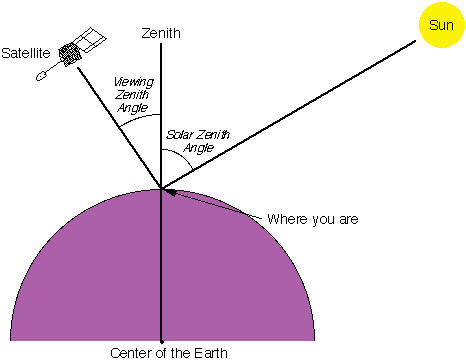
\includegraphics[width=0.6\textwidth]{Figures/ZenithAngles.png}
      \caption{Solar and viewing zenith angles, image copied from \citet{SZA_Image}, originally from a NASA website.}
      \label{ch_HCHO:fig:zenithangle}
    \end{center}\end{figure}

    We use $\nabla I = I_B - I_{B_0}$ to represent the change in intensity due to the absorber. Note that for optically thin absorption, $\nabla I / I_B << 1$, and we can use:
    \begin{equation} \label{ch_HCHO:eqn:AMFthin}
      AMF = \frac{\ln{ \left( 1 - \frac{\nabla I}{I_B} \right)} }{\tau_v} \approx \frac{ - \frac{\nabla I}{I_B} }{\tau_v}
    \end{equation}
    $\nabla I$ can also be expressed as the integral of the absorption slices over optical depth increments: 
    \begin{equation*}
      \nabla I = \int_0^{\tau_v}{\frac{\partial I_B}{\partial \tau} \mathrm{d}\tau}
    \end{equation*}
    which can be placed into equation \ref{ch_HCHO:eqn:AMFthin}:
    \begin{equation*}
      AMF \approx \frac{-1}{\tau_v} \int_0^{\tau_v}{\frac{\partial \ln{I_B}}{\partial \tau} \mathrm{d}\tau}
    \end{equation*}
    and rewritten as:
    \begin{equation} \label{ch_HCHO:eqn:AMFcross}
      AMF = \frac{-1}{\tau_v} \int_0^\infty {\frac{\partial \ln{I_B}}{\partial \tau} \alpha(z)\eta(z)\mathrm{d}z}
    \end{equation}
    where $\alpha(z)$ and $\eta(z)$ represent absorption cross section in m$^2$ molecule$^{-1}$, and number density in molecules m$^{-3}$ respectively. This uses the attenuation cross section relationship to optical depth (see section \ref{ch_HCHO:sec:satelliteHCHO:crosssection}).

    To represent an average cross section weighted by the absorbing species' vertical distribution, intended to account for temperature and pressure dependence of $\alpha(z)$, $\alpha_e$ is defined as:
    \begin{equation*}
      \alpha_e = \frac{1}{\Omega_v} \int_0^\infty \alpha(z) \eta(z) \mathrm{d}z
    \end{equation*}

    This is the same as $ \tau_v = \Omega_v \alpha_e $, which we can place into equation \ref{ch_HCHO:eqn:AMFcross} to obtain:
    \begin{equation*}
      AMF=-\int_0^\infty{ \frac{\partial \ln{I_B}}{\partial \tau} \frac{\alpha(z)}{\alpha_e} \frac{\eta(z)}{\Omega_v} \mathrm{d}z }
    \end{equation*}

    Defining w(z) as the scattering weights describing the sensitivity of the backscattered spectrum to the abundance of an absorber at altitude z:
    \begin{equation}
      \omega(z) = -\frac{1}{AMF_G} \frac{\alpha(z)}{\alpha_e} \frac{\partial \ln{I_B}}{\partial \tau}
    \end{equation}
    and vertical shape factor S$_z$(z) representing a normalized vertical number density profile: 
    \begin{equation} \label{ch_HCHO:eqn:ShapeFactor}
      S_z(z) = \frac{\eta(z)}{\Omega_v}
    \end{equation}
    
    Now the AMF can be expressed as
    \begin{equation} \label{ch_HCHO:eqn:AMFintwSdz}
      AMF = AMF_G \int_0^\infty w(z) S_z(z) \mathrm{d}z
    \end{equation}
    It's worth noting that in the OMI satellite product, the provided $\omega(z)$ term does not include the $\frac{1}{AMF_G}$ term and a the calculation in equation \ref{ch_HCHO:eqn:AMFintwSdz} does not use the $AMF_G$ term.
    This is not noted in any of the papers which recalculate the AMF from the OMI product, due to them recalculating the $\omega$ term themselves with a radiative transfer model such as LIDORT.
    
    For this equation $\omega$ is a function of atmospheric scattering which can be calculated using an RTM to determine the absorption cross section and optical thickness along the path.
    S$_z$(z) can be calculated using an apriori vertical profile, which may be sourced from any atmospheric chemistry model.
    Note that for level two non-gridded OMI satellite HCHO total column data, the w(z), S$_z$(z), and AMF$_G$ are all provided.
    
    Mie scattering and clouds can complicate the calculation of $\omega$(z), however tables of values for this function at various parameter inputs can be used with modeled vertical shape factors for local AMF calculations.
    
    Using the vertical coordinate sigma ($\sigma$), which is related to pressure (P) by $P=\sigma \left( P_S - P_T \right) + P_T$, where subscripts S and T represent earth surface and top of the atmosphere respectively.
    The hydrostatic relation $P = - \rho_a g z$, with $\rho_a$, g, being density of air, gravity, respectively lets us switch to the sigma coordinate using:
    \begin{align*}
      \rho_a g z & = \sigma \left( P_S - P_T \right) + P_T \\
      \mathrm{d}\sigma  & = - \frac{ \rho_a g }{ P_S - P_T } \mathrm{d}z
    \end{align*}
    
    Substitution into \ref{ch_HCHO:eqn:AMFintwSdz} gives AMF using the sigma coordinates:
    \begin{equation} \label{ch_HCHO:eqn:AMFintwSdsigma}
      AMF = AMF_G \int_0^1 w(\sigma) S_\sigma(\sigma) \mathrm{d}\sigma
    \end{equation}
    Where S$_\sigma$ is defined as a vertical shape factor representing a normalised mixing ratio:
    \begin{equation}
      S_\sigma (\sigma) = \frac{\Omega_a}{\Omega_v}C(\sigma)
    \end{equation}
    where $\Omega_a$ is the vertical column of air and C($\sigma$) is the mixing ratio of the absorber.
    This normalised shape factor is dimensionless.
    This can be useful when running global atmospheric models as the ground altitude is always at $\sigma=1$ and we need not worry about topography.
    
    When comparing satellite observations to a chemical model, one needs to recalculate the satellite AMF using their own modelled vertical gas profiles as the a-prior shape factor in order to remove any total column bias which may be due to the satellite's apriori.
    Another way of removing this bias is through deconvolution (TODO: EQNS) of the averaging kernal (AK) of the satellite instrument.
    The AK represents sensitivities to each species at multiple altitudes through the atmosphere and in the case of OMI, can be approximated from the scattering weights ($\omega(z)$) function as follows:
    \begin{equation} \label{ch_HCHO:eqn:AKfromw}
      AK(z) = \frac{\omega(z)}{AMF}
    \end{equation}
    Note that this is an approximation for the OMI product, which does not include the AK but does include the $\omega$ and AMF, as explained in \citet{Abad2015}.
    
  \subsection{Uncertainty in OMI total columns}
  \label{ch_HCHO:sec:OMIuncertainty}
    Provided with the OMI product is the measurement of uncertainty in each pixel, calculated by SAO from the backscattered solar radiation fit \citep{Abad2015,Abad2016}.
    BIRA use another method, and calculate the standard deviation of HCHO over the remote pacific ocean as the uncertainty \citep{DeSmedt2012, DeSmedt2015}.
    In the remote pacific, it can be assumed that HCHO variations are weak, with concentrations remaining steady in the short term ($\sim 1$ month).
    This means the standard deviation over this region can be used as a proxy for determination of the instrument error.
    For an analysis of the uncertainty in the recalculation of the OMI HCHO vertical columns see section \ref{ch_HCHO:sec:OMI_uncertainty_calculation}.
    
  \subsection{Reference sector correction for comparison of products to various models}
    HCHO products from OMI and SCIAMACHY both use a median daily remote pacific ocean radiance reference spectrum, over 15$^{\circ}$S-15$^{\circ}$N, 140$^{\circ}$-160$^{\circ}$W where it is assumed that the only significant source of HCHO is methane oxidation \citep{DeSmedt2008,Barkley2013,Kurosu2014}.
    Since this oceanic background is used instead of a solar irradiance spectrum, in order to compare the output against different models, the vertical columns need to be corrected by an absolute amount.
    The corrected vertical column ($\Omega_V$) is calculated as the slant column ($\Omega_S$) minus the reference slant column ($\Omega_{S_0}$) multiplied by the AMF, plus the modelled reference sector column ($\Omega_{V_B}$):
    \begin{equation*}
      \Omega_V = \frac{ \left( \Omega_S - \Omega_{S_0} \right) }{ AMF } + \Omega_{V_B}
    \end{equation*}
    This method is used in various papers, including \citet{DeSmedt2008, DeSmedt2012, DeSmedt2015, Barkley2013, Bauwens2016}.
    
    Recently this correction was expanded (for OMI data) to include latitudinal and instrument track influence by \citet{Abad2015}.
    The updated correction is explained in detail in section \ref{ch_HCHO:sec:RSC}.
    
%----------------------------------------------------------------------------------------
%	BVOC FROM HCHO SECTION
%----------------------------------------------------------------------------------------
\section{Recalculating HCHO from satellite(OMI) data over Australia}
\label{ch_HCHO:sec:creatinginventory}

  \subsection{Process Outline}
    First satellite slant columns of formaldehyde for the years January 1st, 2005 - April 1st, 2013 are downloaded from NASA.
    The data set used is from the Ozone Monitoring Instrument (OMI) on board the Aura satellite, as it has data for the entire time line and sufficiently covers the southern hemisphere.
    This data is first quality assured and undergoes basic analysis and filtering criteria as is done in several other studies \citep[eg.]{Marais2012, Barkley2013, Bauwens2016, Zhu2016}.
    This filtering removes cloudy and uncertain data points, along with instrument problems such as the OMI row anomaly (see section \ref{ch_HCHO:sec:OMIFiltering}.
    A full account of the filters used when reading OMI satellite data is given in section \ref{ch_HCHO:sec:OMIFiltering}.
    
    In order to reduce uncertainty and increase the utility of the satellite data we regrid it from pointwise single time data points to 8-day averages on a latitude longitude grid which matches our model input and output grid spacing. 
    Using the 8-day average reduces the uncertainty in each datapoint significantly, TODO: citet marais and barkley uncertainty improvements, details of the uncertainty estimations is shown in section \ref{ch_HCHO:sec:OMI_uncertainty_calculation}.
    %Another example is shown in \citet{Vigouroux2012} where uncertainty near a specific location is lowered by averaging daily within a 500km radius and only using the meaned data when there are at least 20 good values.
    
    Once the slant columns are quality filtered and gridded, additional data sources need to be used to account for anthropogenic and pyrogenic sources of HCHO.
    MODIS fire counts are used in conjunction with NO$_2$ enhancements (also measured by satellite) to remove data points which may be affected by fires. 
    TODO:If it is easier to use OMI smoke smoke aaod I'll do it that way instead of using the NO2, write here if that is the case.
    One possible solution to anthropogenic filtering is the national pollution index (TODO:cite:\verb|http://www.npi.gov.au|) which contains industrial HCHO and NO$_X$ emissions from 2003 to 2014.
    This has a negative affect on uncertainty, as fewer measurements are averaged over the 8-days. 
    The affect of the fire filtering on uncertainty, and how many points are removed is shown in section \ref{ch_HCHO:sec:filteringfires}.
    
    Each satellite slant column measurement is corrected by some amount, based on the divergence from a modeled reference sector.
    The reference sector correction method corrects for several problems, however it introduces some apriori model influence.
    One of the problems removed through this correction method is instrument degradation, which can introduce bias over time.
    Another is the possible influence of varying dead/hot pixel masks across 2-D detector arrays such as OMI \citep{DeSmedt2015}.
    This method also corrects for the errors introduced through correlations between BrO and HCHO absorption cross sections, which are especially significant at high latitudes \citep{Abad2015}.
    
    The reference sector we use is defined over the pacific ocean at 140 to 160$^{\circ}$W and 90$^{\circ}$N to 90$^{\circ}$S, as in \citet{Abad2015}.
    HCHO concentrations are assumed to be at background levels over the pacific ocean, with their only source being CH$_4$ oxidation.
    A correction for each instrument pixel is created based on the difference between the background HCHO measurements from OMI and the GEOS-Chem modelled HCHO columns within the reference sector.
    This correction is calculated daily and applied to all good pixels based on their latitude.
    The full process for this is shown in section \ref{ch_HCHO:sec:RSC}.
    
    In order to visualise and analyse satellite column data it is generally transformed into vertical columns. 
    This is done using AMF calculations as shown in section \ref{ch_HCHO:sec:satelliteHCHO:CalculationOfVC}.
    Taking the biogenic slant columns, scattering weights, and apriori estimates of HCHO vertical profiles we determine vertical HCHO column amounts.
    This is an in depth process involving radiative transfer modelling in order to work out satellite sensitivities at various altitudes, as well as the effect from the local HCHO profile on those sensitivities.
    Several of these required data are available from the satellite data products, including the scattering weights and the zenith angles required to determine an AMF at any particular measured point.
    In this work the shape factor is recalculated from GOES-Chem, with the associated OMI per-pixel scattering weights unchanged. 
    The satellite shape factor is replaced by GEOS-Chem's overpass time simulated HCHO profile, normalised and saved daily along with air density.
    
    When comparing satellite measurements against models it is important to recognise the impact of the apriori shape factor on the total column values.
    This is due to the sensitivity of instruments varying vertically through the atmosphere, and how the simulated distribution of HCHO is accounted for.
    In order to remove a possible bias caused by systematic differences between the old model and the current model, the shape factor used by the satellite is replaced using the profile from the current model before satellite total columns are recalculated (generally using equation \ref{ch_HCHO:eqn:AMFintwSdz}).
    Both the shape factor and scattering weights of the satellite are recalculated using a combination of GEOS-Chem apriori profile information and satellite measurement data using code initially written by dr. Paul Palmer, which calculates the AMF after running the LIDORT radiative transfer calculations to determine apriori scattering, this is explained fully in section TODO: and how it's used is shown in section \ref{ch_HCHO:sec:PPCode}.
    Without performing this step a bias between modeled and measured total column values may be due to an apriori rather than actual chemistry or measurements.

  \subsection{Quality filtering OMI HCHO slant columns}
    \label{ch_HCHO:sec:OMIFiltering}
    TODO: Quality flags and cloud cover metric uses, and discussion, along with statistics like how many datapoints are removed.
    
    The OMI dataset has a quality flag which can be used to remove unlikely or poor satellite measurements.
    The states represented by this quality flag are shown in table \ref{ch_HCHO:tab:OMIQualityFlag} which is taken from \citet{Kurosu2014}.
    Filtering bad or missing measurement pixels is preformed prior to any other filtering, this includes the datapoints affected by the row anomaly.
    This anomaly (\url{http://projects.knmi.nl/omi/research/product/rowanomaly-background.php}) affects radiance data at particular viewing angles, corresponding to a row on the CCD detectors, and is dynamic over time.
    The slant columns affected are flagged and easy to remove before further processing.
    
    Clouds have various detrimental effects on slant column uncertainty and AMF calculation, so the cloudy data needs to be filtered.
    Any pixel with a cloud fraction of greater than 40\% is also removed, after the pixel is used in determining the reference sector correction, as is done in \citet{Abad2015, DeSmedt2015}.
    %In \citet{???} (TODO: find this paper), pixels with more than half of the backscattered intensity from the cloudy sky fraction are removed, in effect removing pixels with more than ~40\% cloud fraction before calculating the AMF for NO$_2$ slant columns.
    Another way this has been performed is to remove pixels where the AMF lies outside a certain range: \citet{Martin2002} filter AMFs below 0.5 in order to remove the effects of heavy cloud and optical thickness.
     
    \begin{table}
      \caption{OMI quality flag values table from \citet{Kurosu2014}}
      \begin{tabular}{  l  l  p{10cm} }
        \hline
        \textbf{Value} & \textbf{Classification} & \textbf{Rational} 
        \\ \hline
        0 & Good & Column value present and passes all quality checks; data may be used with confidence. 
        \\ \hline
        1 & Suspect & Caution advised because one or more of the following conditions are present: 
          \begin{itemize}
            \item Fit convergence flag is $<$ 300 but $>$ 0: Convergence at noise level
            \item Column $+ 2 \sigma$ uncertainty $<$ 0 $<$ Column $ + 3 \sigma $ uncertainty
            \item Absolute column value $>$ Maximum column amount (1e19 molec cm$^{-2}$)
          \end{itemize}
        \\ \hline
        2 & Bad & Avoid using as one of the following conditions are present: 
          \begin{itemize}
            \item Fit convergence flag is $<$ 0 : No convergence, abnormal termination
            \item Column $+ 3 \sigma$ uncertainty $<$ 0
          \end{itemize}
        \\ \hline
        $<0$ & Missing & No column values have been computed; entries are missing
        \\ \hline
      \end{tabular}
    \label{ch_HCHO:tab:OMIQualityFlag}
    \end{table}
    
    The cloud fraction with each pixel is provided with the OMHCHO dataset, however its source is the OMI cloud product, OMCLDO2.
    To give an idea of how much data is filtered out, around 30\% of the pixels which remain after filtering out the bad or missing data are subsequently removed due to cloudiness.
    
    Further filtering is performed to remove the measurements which are most likely to be unrealistic: pixels wit a solar zenith angle greater than 60$^\circ$, and those with column density outside the range $-0.5 \times 10^{16}$ to $10^{17} $~molecules cm$^{-2}$.
    These are similar filters to those applied in (TODO: read \citet{Zhu2016}, add similar justification if succinct).
    This final filter is required due to currently unexplained large negative values which occur in the OMI HCHO product increasingly over time.
    Figure \ref{ch_HCHO:fig:OMI_negative_hist} shows how unfiltered HCHO columns are affected by a small set of highly negative values which heavily affect the mean column amount over any region.
    The histograms here show the negative (left) and positive (right) total column HCHO measurements from a subset of swaths over Australia, on the 18th of March 2013.
    The highly negative values can be seen around the $-10^{19}$~molecules cm$^{-2}$ region.
    
    \begin{figure}[!htbp]\begin{center}
      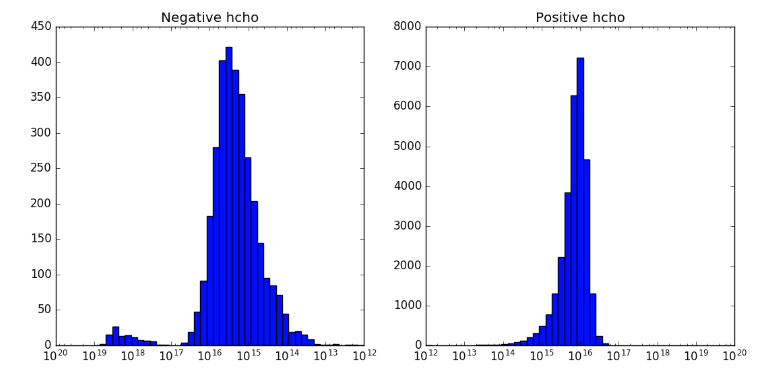
\includegraphics[width=0.7\textwidth]{Figures/AusOMHCHO_Hist_20130318.png}
      \caption{Column density histograms for a subset of OMI swaths over Australia on the 18th of March 2013.
      Negative entries are shown in the left panel, positive in the right, note the different scale between negative and positive panels.}
      \label{ch_HCHO:fig:OMI_negative_hist}
    \end{center}\end{figure}
    
    One final selection of the data is removed prior to calculation and analysis due to instrument sensitivity issues.
    This removed data is based on the latitude of the satellite measurement, high northern and southern latitudes are removed as the effect of both the high solar zenith angle and (over arctic regions) the high albedo cause anomalous readings which are hard to correct.
    The latitudes removed from analysis for OMI satellite data are those outside of $0^\circ \pm 60^\circ$. 
    This is where the satellite measurements are less robust, and often publications will remove this same region (TODO: cites where they did this).
  
    
  \subsection{Reading OMHCHO daily slant columns}
    Each $\sim90$ minutes the AURA satellite sweeps over the sunny side of the planet, with OMI recording roughly 90~k pixels, of which around 50~k -- 80~k are classified as good.
    Each pixel contains several important pieces of data which are needed for recalculation of the HCHO vertical column: the total column of HCHO (molecules cm$^{-2}$), cloud fraction, associated shape factor, AMF, geometric AMF, scattering weights and their vertical altitudes (hPa), viewing zenith angle, solar zenith angle, latitude, longitude, OMI sensor track, main data quality flag, cross track flag, and total column uncertainty.
    All of these data are needed in order to reconstruct the total vertical column using a modelled apriori shape factor rather than NASA's included apriori shape factor.
    Each pixel and it's relevant data are saved in a long list, around $1.1$ million pixels per day.
    As well as the data directly read from the OMI swath files, further information is added to each pixel.
    This is the new AMF calculated through replacing the apriori vertical profile with the newer GEOS-Chem simulated profile, which is described in section \ref{ch_HCHO:sec:recalculating_AMF_description}.
    The shape factors and scattering weights for each pixel lie along a z-axis which is vertically resolved to 47 layers and is shown in figure TODO: make figure showing this stuff and an example profile.
    
    TODO: Show an example of OMI swaths.
    
  \subsection{Regridding to 0.25 by 0.3125 8-day averaged vertical columns}
    
    Regridded OMI HCHO columns from the are based on 14-15 daily swaths of measurements provided by NASA. 
    Each swath contains roughly $9 \times 10^4$ pixels, each of which contains various data including latitude, longitude vertical column HCHO, etc.
    In order to regrid these columns each pixel is mapped into a global grid of 0.25$^{\circ}$x0.3125$^{\circ}$ latitude by longitude (matching GEOS-5 native resolution) which may contain up to 15 entries from a particular day's orbits.
    Total vertical column amounts (both the satellite original and the columns reprocessed as follows) are averaged over each 8 days starting on January 1st 2005.
    
    The process of regridding is performed by first reading all relevent information at each pixel for a single day into a list in python, which is then processed, with the shape factor read from GEOS-Chem output and AMF recalculated, before being saved as a gridded array of total columns and pixel counts.
    The total columns are averaged into each grid box for each day, and eventually averaged over eight day time periods.
    
    TODO: time per regridding and reprocessing:
    This mapping requires some processing time as well as RAM and computer storage space, and has been performed on the National Computing Infrastructure (NCI) supercomputer cluster.
    In order to reprocess one year of swath files, X GB of daily data was downloaded and then transformed into Y GB of 8-day averaged gridded data.
    This takes around 90 minutes per day, and is very parallelisable as each day is completely independent.
    Using N$\times 8$ concurrent processors on NCI's computer cluster running Python allows for very fast reprocessing of our entire timeline.
    As much as possible, processing is done using the HDF-EOS5 format, with GEOS-Chem output being read and processed from bitpunch to HDF-EOS5 prior to reprocessing.
    The scripts to regrid and reprocess the swath data set are available in the supplementary (TODO).
    
  \subsection{Filtering pyrogenic HCHO}
  \label{ch_HCHO:sec:filteringfires}
    TODO: How modis fire counts are used as well as statistics on removed data points.
    
    On board NASA's AQUA satellite, the MODIS instrument is used to detect fire activity.
    The product used here is called MYD14C8H (\citep{Giglio2006}), which looks at fire activity over eight days on a 0.5$^{\circ}$ square grid globally.
    Regridding the product to the native meteorological grid of GEOS5 at 0.25$^{\circ}$ latitude by 0.3125$^{\circ}$ longitude is done in python with an interpolator which maps the values of the new grid rectangles to the value of the nearest grid square.
    An example of the change in resolution is provided in figure \ref{ch_HCHO:fig:modisgridspace}, where the grids are shown over a basic map of Tasmania.
    The direct affect of this interpolation is shown as an example in figure \ref{ch_HCHO:fig:modisinterpolation}, which is showing the regridded MODIS fire count over Australia from January 2005 (avg of first 8 days) in two subplots.
    
    \begin{figure}[!htbp]\begin{center}
      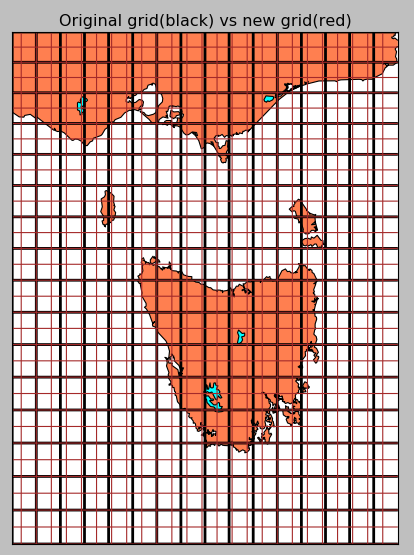
\includegraphics[width=0.7\textwidth]{Figures/MODIS_grid_space.png}
      \caption{Example of grid space change using 0.5x0.5 and 0.25x0.3125 latitude by longitude resolution.}
      \label{ch_HCHO:fig:modisgridspace}
    \end{center}\end{figure}
    
    \begin{figure}[!htbp]\begin{center}
      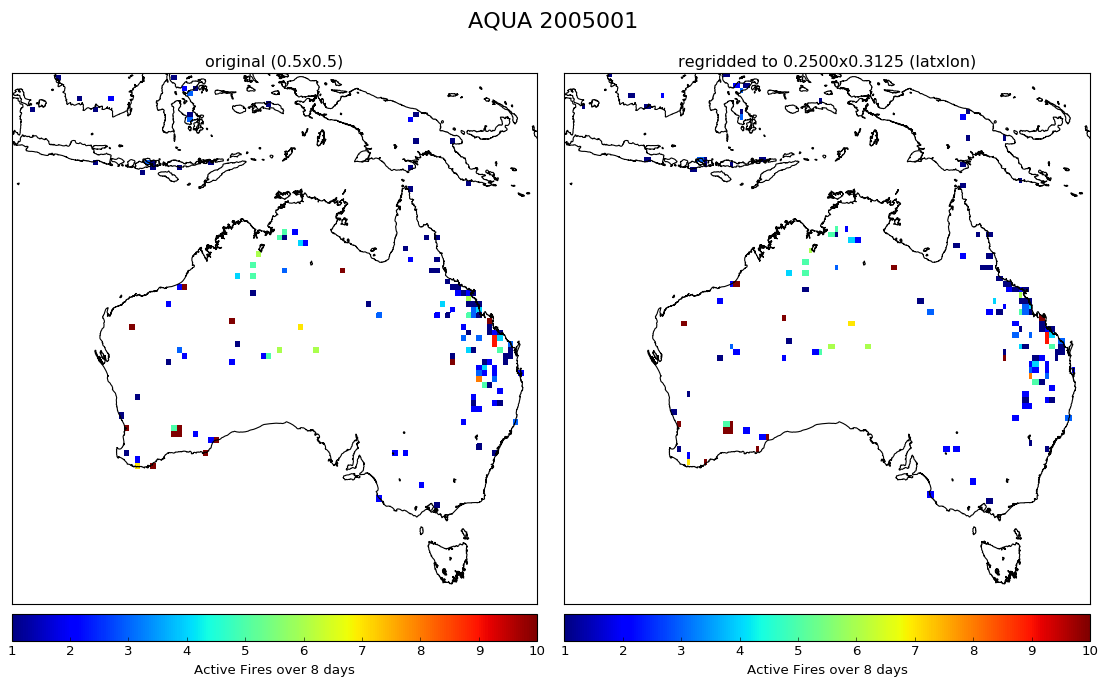
\includegraphics[width=\textwidth]{Figures/MODIS_Regrid_Comparison.png}
      \caption{Example of MODIS 8 day grid interpolation from 0.5x0.5 to 0.25x0.3125 latitude by longitude resolution.
      This example uses MODIS fire counts for 1-8 January 2005.}
      \label{ch_HCHO:fig:modisinterpolation}
    \end{center}\end{figure}
    
    Figure \ref{ch_HCHO:fig:fireexclusionexample} shows an example of the total column HCHO calculated using GEOS-Chem aprioris ($\Omega_{GEOS}$) before and after using the MYD14C8H product to exclude fire influenced pixels.
    (TODO: show time series of how many pixels are removed and discuss if this causes any issues down the line)
    % January 1, 2005 : 113384 / 130295 nan entries before and after fire exclusion within 60 degrees of equator
    
    \begin{figure}[!htbp]\begin{center}
      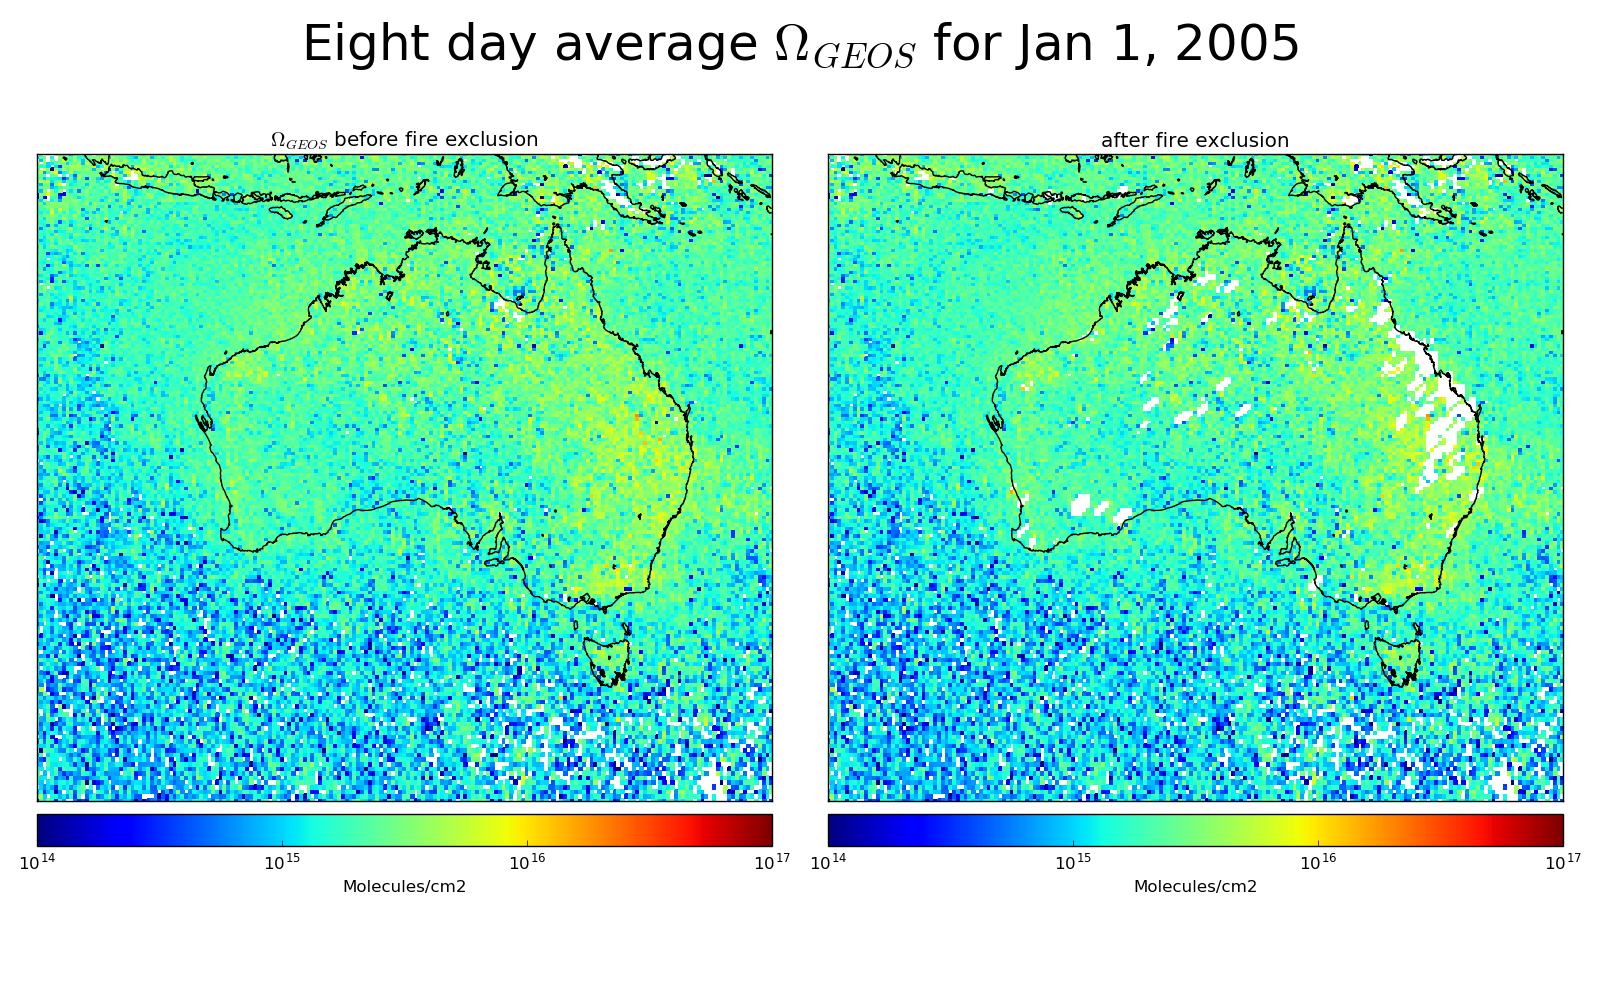
\includegraphics[width=\textwidth]{Figures/HCHO/fire_exclusion_aus_8d.png}
      \caption{Vertical column HCHO calculated using OMI satellite swaths with GEOS-Chem aprioris, averaged over 1-8 January 2005 with and without fire affected squares removed.}
      \label{ch_HCHO:fig:fireexclusionexample}
    \end{center}\end{figure}
    
    This filtering ends up removing too much information, and the recalculation of HCHO is too negatively influenced.
    To deal with this a separate product from the same instrument has been downloaded: MYD14A1, which keeps daily fire counts.
    Less disruptive filtering can be achieved by removing pixels which coincide with fires on the same day, as shown in figure TODO: which compares the 8 and 1 day filtering.
    TODO: The script to read and regrid these one day fire counts was adapted from X.
    Figure (TODO: effect on uncertainty and time series of fire pixels removed) shows the daily filtering effect on uncertainty and time series of fire pixels removed.
    
  \subsection{Filtering anthropogenic HCHO}
    TODO
  
  \subsection{Recalculating the AMF to create our own vertical HCHO columns}
  \label{ch_HCHO:sec:recalculating_AMF_description}
    OMI's apriori shape factor is based on the GEOS-Chem (v9) model, which uses 47 layers between the earth's surface and the top of the atmosphere using a pressure-eta hybrid (the actual values are shown in table \ref{app_a:tab:gc_47_vgrid}).
    Taking a more recent GEOS-Chem apriori shape factor and integrating along the vertical axis using equation \ref{ch_HCHO:eqn:AMFintwSdz} gives us a new AMF (AMF$_n$).
    Since we are using the $\omega$ provided by OMI, we remove the AMF$_G$ term from this calculation.
    The integration is done in Python using a simple rectangular method, which multiplies the integrand midpoints by the change in height, and then takes the sum.
    This is identical to calculating the integral if we assume the integrand is linear between each measured point, and introduces no new uncertainty.
    All that remains for recalculating the total vertical column using our new apriori shape factor is to apply the new AMF and remove the old:
    \begin{equation*}
      \Omega_{new} = \Omega \frac{AMF}{AMF_n}
    \end{equation*}
    
    The vertical column scattering weights and apriori shape factors provided in the OMHCHO dataset are defined on 47 levels.
    In order to reformulate the vertical column using updated GEOS-Chem hcho apriori shape factors I have run GEOS-Chem version 10.01 on the full 72 level vertical grid at 2 by 2.5 (lat by lon) degree monthly resolution. 
    The simulated vertical profiles of HCHO are averaged from 1300-1400 local time in order to match the satellite overpass time of roughly 1330.
    These vertical profiles then provide the apriori shape factor for the higher horizontally resolved satellite columns, which pick the nearest apriori from the model.
    TODO: determine which of these is correct!
    a)The new apriori profiles are monthly averages, which is the same temporal resolution used by the OMI apriori shape factors.
    b)The new apriori profiles are simulated daily and averaged over 8 days along with the recalculated total vertical columns.
    
    A new AMF is determined using equation \ref{ch_HCHO:eqn:AMFintwSdz}) with the apriori shape factor set by our GEOS-Chem model run.
    In order to reformulate the AMF, GEOS-Chem's 72 level vertical profile is transformed from ppb to a normalized number density profile in order to match equation \ref{ch_HCHO:eqn:ShapeFactor}. 
    This conversion uses the following equation: 
    \begin{equation} \label{ch_HCHO:eqn:ppbto}
      \eta_{HCHO} = ppb_{HCHO} \times \eta_a \times 10^{-9}
    \end{equation}
    where $\eta_{HCHO}$ is the number density of a HCHO, and ppb$_{HCHO}$ is the molecules of that species per billion molecules of air.
    In order to normalize these vertical density profiles over the globe, we divide by the modelled total vertical column $\Omega_{HCHO}$ which is determined by:
    \begin{equation*}
      \Omega_{HCHO} = 2.12\times 10^{13} \Sigma_z \left( ppb_{HCHO}(z) (P(z)-P(z+1)) \right)
    \end{equation*}
    where P(z) is the pressure (hPa) at the bottom of altitude level z, the constant 2.12e13 is determined from equation (TODO: run through this number in another section?).
    In effect this equation sums over the molecules per cm$^2$ in each altitude level.
    
    We have S$_z(z)$ and $\omega(z)$ over the vertical pressure coordinate z at all latitude and longitude points on whatever grid we wish. 
    A conversion to the sigma ($\sigma$) vertical coordinate is performed using $ P = \sigma (P_S - P_T) + P_T$, where $P_T$ is pressure at the top of the atmosphere and $P_S$ is surface pressure.
    In the sigma coordinate system we calculated the shape factor as follows:
    \begin{equation} \label{ch_HCHO:eqn:ShapeFactorSigma}
      S_\sigma(\sigma) = \frac{\Omega_a}{\Omega_v}C_{HCHO}(\sigma)
    \end{equation}
    where $\Omega_a$ is the vertical column of air from the surface to the top of the atmosphere and C$_{HCHO}(\sigma)$ is the mixing ratio of HCHO.
    This equation comes from \citet{Palmer2001}, and is unitless since $\Omega_a / \Omega_v$ is molecules of air per molecule of HCHO; the opposite of $C_{HCHO}$.

    Pressure dimension from OMI are the surface pressures from each gridbox (offline conversation with Dr Christopher Miller).
    Determining the geometric pressure midpoints (here onwards pressure levels) and interpolating to our increased vertical resolution involves a few steps.
    The lowest level (with highest pressure) in whichever pressure dimension (ours or OMI's) extends to the lowest altitude (or highest pressure) is interpolated upwards to match the lowest level in the other dimension.
    Secondly, if the OMI dimension has been changed, the scattering weights are interpolated onto this updated dimension.
    Figure \ref{ch_HCHO:fig:AMF_Surface_Relevel} shows how these first two steps are applied using three fake array comparisons and updating the array with the lower surface level.
    Finally, once our dimensions match at the surface (we are not so worried about the very top of the atmosphere) we interpolate the scattering weights onto our updated GEOS-Chem pressure dimension.
    
    \begin{figure}[!htbp]
      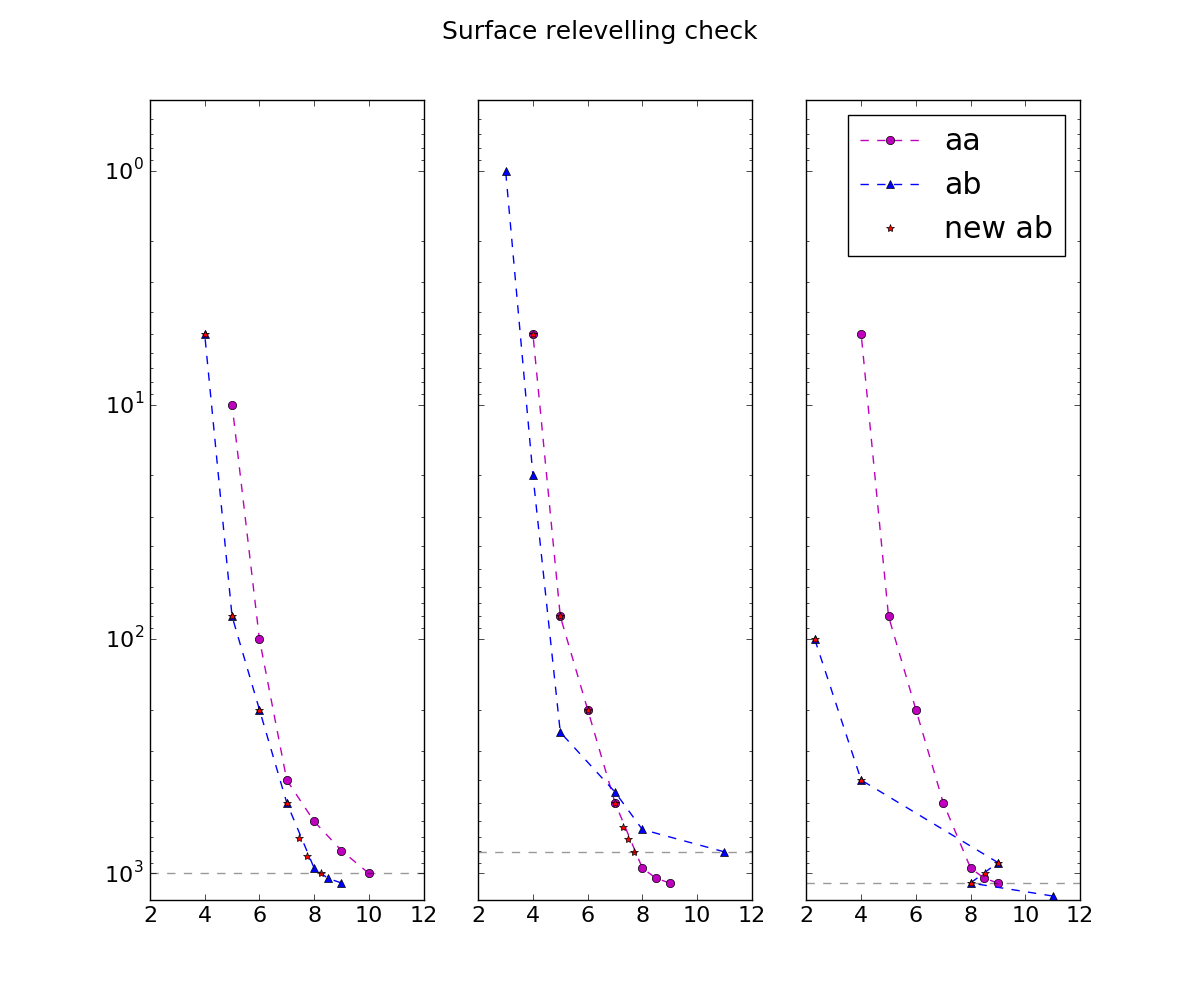
\includegraphics[width=\textwidth]{Figures/HCHO/SurfaceRelevelCheck.png}
      \caption{Constructed example of the initial interpolation of OMI's $\omega$ onto a pressure dimension with mismatched surface pressure.}
      \label{ch_HCHO:fig:AMF_Surface_Relevel}
    \end{figure}
    
    %If I change this to use an inverted geometric midpoint calculation then I need to explain it, otherwise I will need to note the assumption
    %$ \sqrt{ \left( P_1 \times P_{surf} \right)} = P_0 $
    %becomes $ P_{surf} = \frac{P_0^2}{P_1} $ where currently I'm using $P_0$ as the surface.

    S$_\sigma(\sigma)$ Is determined after running GEOS-Chem, which outputs vertical profiles of air density and HCHO mixing ratio, at 72 vertical levels with associated metadata such as vertical layer height and pressure, grid box location, height, and surface pressure.
    Using these outputs the vertical columns ($\Omega_a, \Omega_v$) are calculated for each horizontal grid point (i, j) as follows:
    \begin{align*}
      \Omega_a(i,j) &=& \Sigma_z \left( N_a(i,j,z) \times H(i,j,z) \right)
      \\
      \Omega_z(i,j) &=& \Sigma_z \left( N_{HCHO}(i,j,z) \times H(i,j,z) \right)
    \end{align*}
    where $N_a$, and $N_{HCHO}$ are the densities of air and HCHO, H is the layer height (for each grid box).
    Note that HCHO density is determined from the outputted mixing ratio: $N_{HCHO} = C_{HCHO} \times N_a$.

    S$_\sigma(\sigma)$ is then stored in HDF-EOS5 format, to be used in conjunction with the satellite measurements to calculate an AMF as shown in equation \ref{ch_HCHO:eqn:AMFintwSdz}.
    As the GEOS-Chem V10.01 output is in bitpunch format, the code to read the data and create the shape factor is written in IDL, which has many procedures and functions which are already written to handle reading this format (provided by GAMAP).
    The code is provided in supplementary TODO: put code into supplement section.
    
    For each OMI slant column, a new AMF is calculated using S$_\sigma(\sigma)$ and the provided scattering weights $\omega(\sigma)$ using equation \ref{ch_HCHO:eqn:AMFintwSdz}.
    This integral is applied in python by taking the sum of S$_\sigma(\sigma) \times \omega(\sigma) \times \mathrm{d}\sigma$ for each $\sigma$ determined at 72 levels in GEOS-Chem, with the provided $\omega$ interpolated linearly to these same levels.
    An example of these interpolations is shown in figure TODO: interpolation figure with symbols at original points and interpolated line overplotted for both functions over hPa.
    Globally this reprocessing changed the AMF by TODO: global total percent difference in AMF. 
    In total this caused TODO: total column HCHO change globally/yearly
    In Summer over Australia the global AMF difference was TODO: Difference summers only.
    This changed Australia's HCHO amounts from TODO: X to Y Tg per year plus minus one std.
    
  \subsection{AMF code from Paul Palmer}
  \label{ch_HCHO:sec:PPCode}
    TODO: describe how I use this here
    I use code originally written by Dr. Paul Palmer with various updates and modifications described in section (TODO:) as another way to recalculate the AMF using information from the satellite swaths and the GEOS-Chem overpass simulation output.
    These are used to recalculate the instrument sensitivity or scattering weights for each pixel, as well as the shape factor which together are integrated to give the pixel AMF.
   
   GEOS-Chem outputs quantities averaged between 1200 and 1400 LT, including optical depths at several wavelengths (TODO: list), dust, and HCHO.
   I run a script on the satellite swaths which pulls out a subset of the pixel information into a daily csv file, which can be read by the AMF code as modified by Dr. Luke Surl, in conjunction with the GEOS-Chem outputs for each day.
   The AMF code is then run and produces a csv of recalculated AMFs which get read by my python code and associated with the corresponding pixel.
    
  \subsection{Determination and application of the pacific ocean reference sector normalisation}
    \label{ch_HCHO:sec:RSC}

    As is done in \citet{Abad2015}, a reference sector defined over the Pacific ocean is used to correct OMI instrument degradation.
    This correction is calculated based on satellite measurements over the pacific ocean reference sector; between 140$^{\circ}$W and 160$^{\circ}$W, covering every latitude.
    Corrections are made using apriori HCHO columns in the same reference sector modelled using GEOS-Chem.
    The apriori reference sector of HCHO vertical columns (VCs) is created by GEOS-Chem using 15 minute time resolution, with 2 by 2.5$^{\circ}$ latitude by longitude resolution.
    These simulated values use the GEOS-Chem output averaged between 1300 and 1400 local time at each grid box, in order to match the overpass time of OMI.
    The longitudinal average is taken within the apriori reference sector, as corrections are assumed to be longitudinally invariant.
    The modeled reference sector is interpolated latitudinally in for use in the OMI measurement correction array creation.
    Figure \ref{ch_HCHO:fig:Summary_RSC} the simulated reference sector VCs as an example, calculated on January 1st 2005.
    In this figure the vertical resolution is increased from 2$^{\circ}$ to 0.36$^{\circ}$, through linear interpolation, in order to form 500 vertical bins which are used in correcting the satellite data.
    Each day, good satellite measurements taken over the reference sector are used to determine a correction array.
    The correction is based on the difference between measured slant column and the modeled slant column within the reference sector.
    The model does not produce slant columns associated with each measurement, however one is created by multiplying the VC with the associated slant column's AMF.
    
    \begin{figure}[!htbp]\begin{center}
      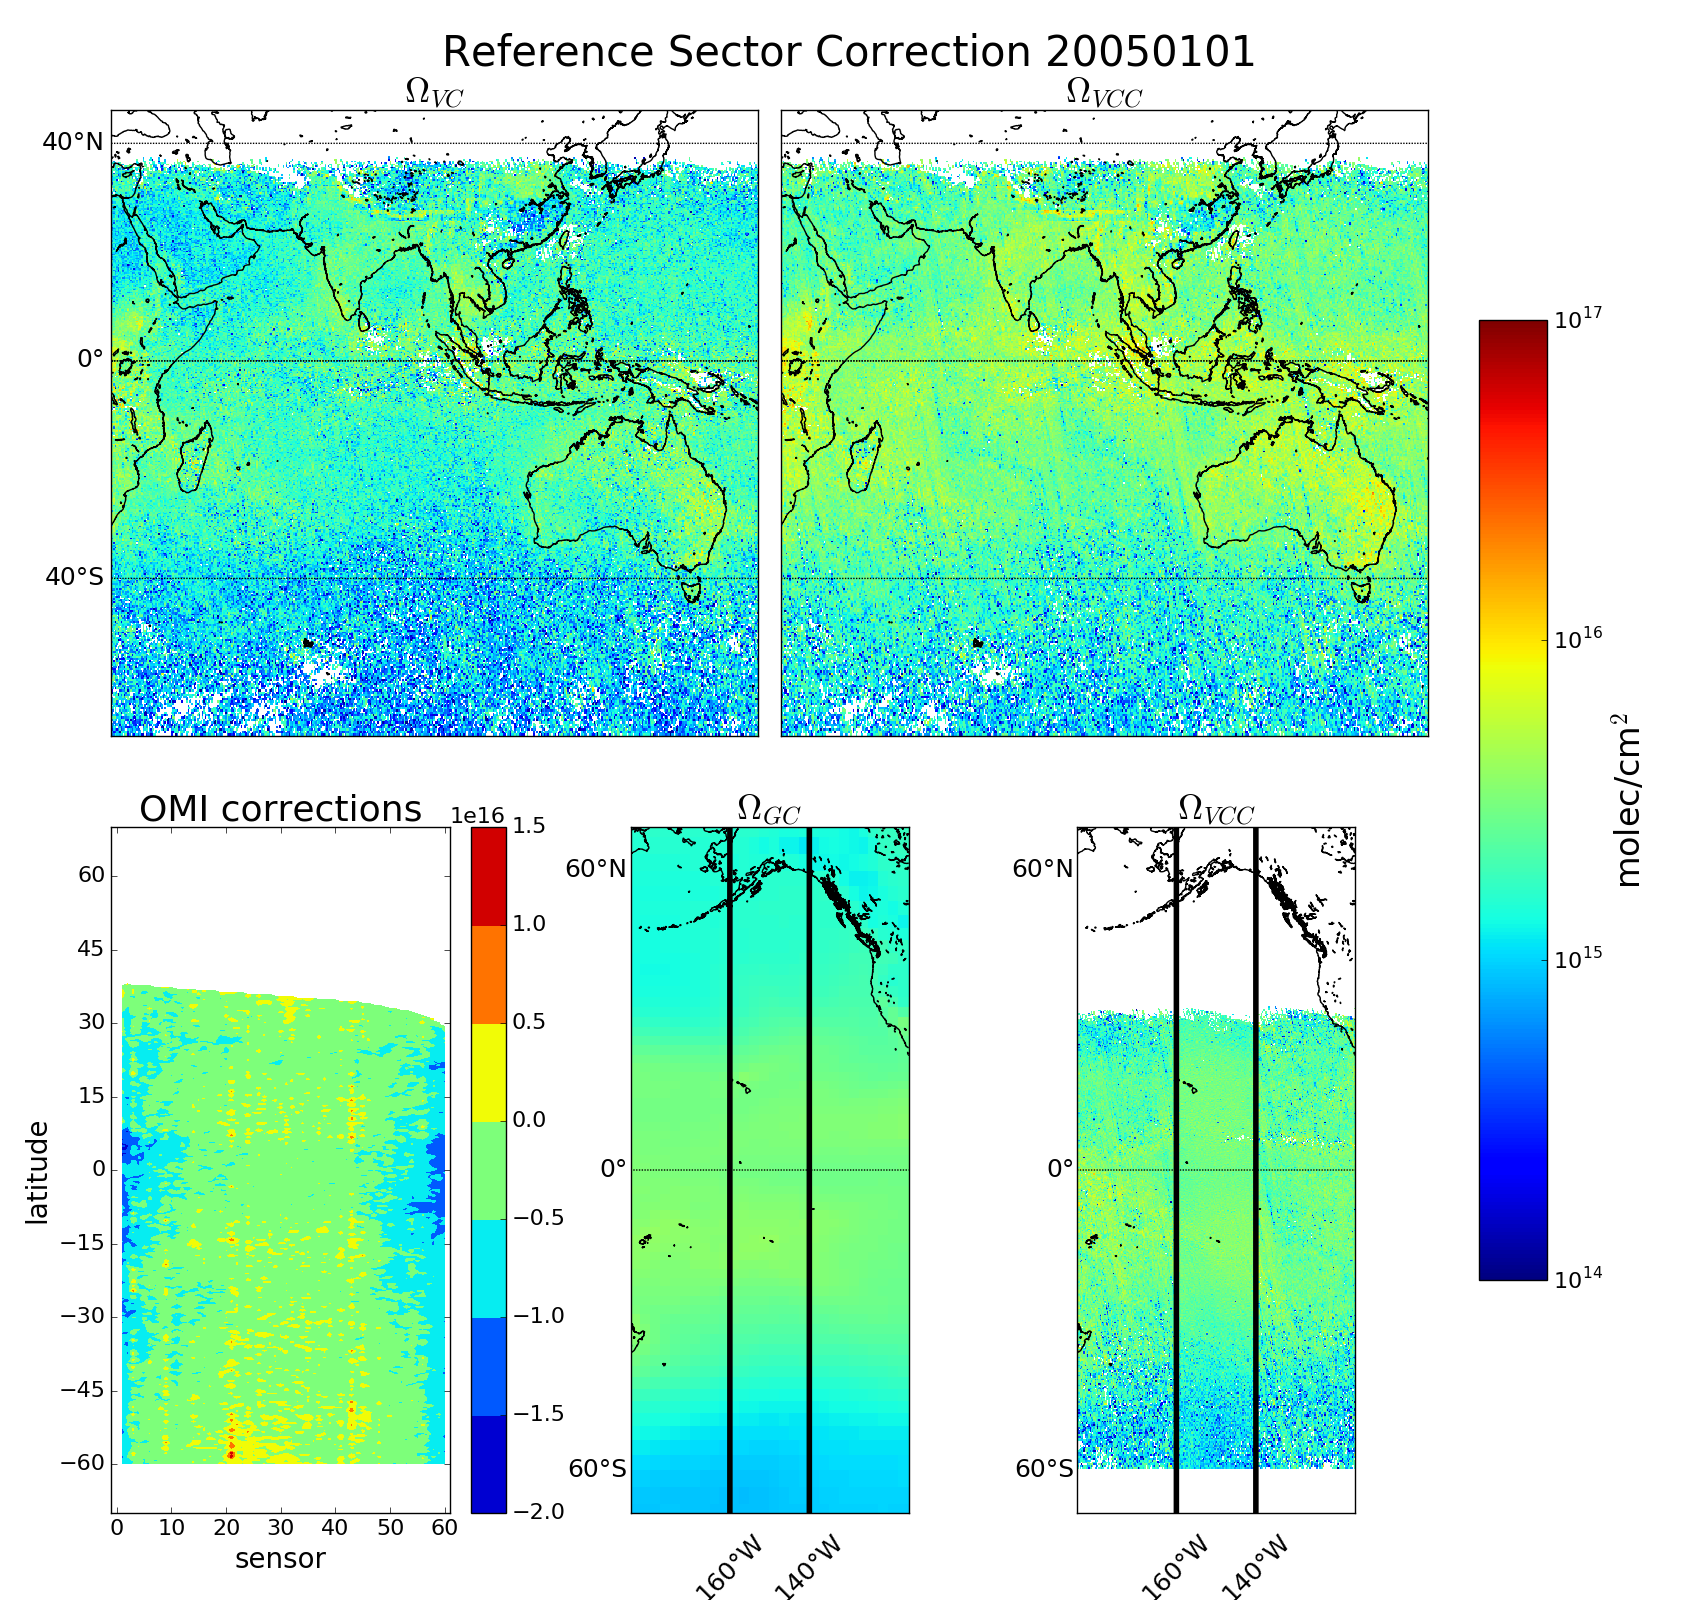
\includegraphics[width=0.7\textwidth]{Figures/HCHO/Summary_RSC_Effect8d_20050101.png}
      \caption{ %
	Example of remote pacific reference sector correction (RSC) using 8-day average measurements and one month modelled data.
	$\Omega_{VC}$ shows the uncorrected vertical columns, while $\Omega_{VCC}$ shows the corrected vertical columns.
	OMI corrections shows the correction applied globally based on latitude and OMI track number(sensor).
	$\Omega_{GC}$ shows the GEOS-Chem modelled HCHO VC over the RSC, with $\Omega_{VCC}$ showing the corrected VC over the same area.
      }
      \label{ch_HCHO:fig:Summary_RSC}
    \end{center}\end{figure}
    
    For OMI swaths, each row of measured data contains 60 `Across track'(track) measurements.
    The track index (i) relates a the measurement to one of the 60 columns of data.
    Corrections for each measurement are calculated by taking the difference between the measured slant column and the apriori slant column as follows:
    \begin{equation} \label{ch_HCHO:eqn:reference_sector_correction}
      Correction(i,j) = SC_{HCHO}(i,j) - VC_{GEOS-Chem}(lat(j)) \times {AMF_{OMI}}(i,j)
    \end{equation}
    where j represents a latitude index and $VC_{GEOS-Chem}(lat)$ represents the apriori reference sector vertical column HCHO at the latitude corresponding to j.
    Note that the correction is in molecules per cm$^2$.
    
    The reference sector correction is independently calculated for each of the 60 tracks, at each latitude where a good satellite measurement exists which used that track.
    The Correction$(i,lat(j))$ function is determined by binning corrections for each track into 500 equidistant latitude bands. 
    
    Due incomplete latitudinal coverage, the correction for each track is interpolated linearly between measurements, with corrections outside of the highest measured latitudes being equal to the corrections at the highest measured latitudes.
    Figure \ref{ch_HCHO:fig:track_correction_interpolations} shows an example of the 60 track corrections for January 1st 2005, the points are satellite measurements and the lines are the interpolations for each track.
    \begin{figure}[!htbp]\begin{center}
      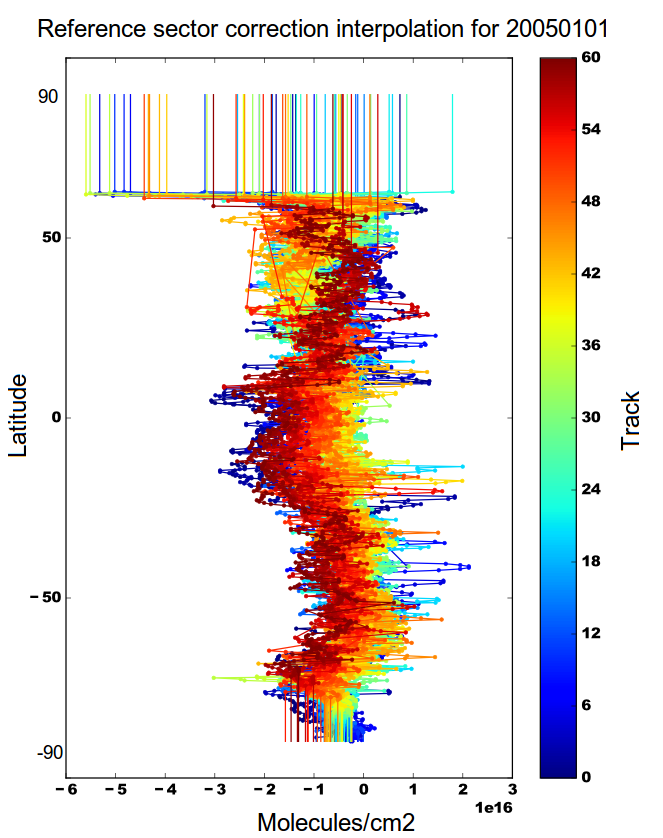
\includegraphics[width=0.7\textwidth]{Figures/HCHO/track_corrections20050101.png}
      \caption{Example of track correction interpolations for January 1st 2005, points represent satellite slant column measurements, with lines interpolating and extrapolating along the latitudinal direction.}
      \label{ch_HCHO:fig:track_correction_interpolations}
    \end{center}\end{figure}
    
    Another way to look at this correction is given in the OMI corrections panel of figure \ref{ch_HCHO:fig:Summary_RSC}, which has the sensors along the x axis, and latitude on the y axis, and shows how for this example 8-day period, the corrections are distributed with more negative values towards the left or right sensors, especially in the tropics.
    
    One correction is associated with every good satellite measurement which is used to create a reference sector corrected measurement (Vertical Column Corrected or VCC) through the following equation:
    \begin{equation}
      VCC(i,j) = \frac{SC_{HCHO}(i,j) - Correction(i,lat(j))}{AMF(i,j)}
    \end{equation}
    Finally, for each day, the good satellite measurements are averaged into our own latitude longitude resolution bins along with the associated corrected SC, VC, VCC, AMF, and bin entry count.
    The bin entry count is used to create an 8-day average out of the one day averages, as it is the daily mean multiplied by the daily count summed over 8 days divided by the total count for each bin.
    
  \subsection{Estimation of error or uncertainty}
  \label{ch_HCHO:sec:OMI_uncertainty_calculation}
    There are three main sources of error in the resulting HCHO columns:
    \begin{description}
      \item[a] Fitting error from the OMI retrieval.
      \item[b] Uncertainty in AMF calculations.
      \item[c] Uncertainty of HCHO background.
    \end{description}

    a) is available in the OMI product and reduced through spatial and temporal averaging.
    Taking the eight day grided average with horizontal resolution of 0.25 by 0.3125 degrees (latitude by longitude) typically reduces uncertainty by a factor of 1.5 to 4.
    Another method for examining uncertainty of OMI is to analyse the standard deviation of the HCHO columns over the remote pacific.
    If we assume there is no HCHO variation from background levels over any 8-day period, then this method infers variations in the measuring instrument, and can be used as a metric for uncertainty as done in \citet{DeSmedt2012}.
    TODO: uncertainty calculation on remote pacific OMI.
    \cite{Millet2006, Palmer2006} both examine OMI HCHO columns over North America and determine overall uncertainty to be 40\%, with most of this coming from cloud interference.

    b) is determined through an analysis of GEOS-Chem output, validated against the total column of HCHO at Wollongong using FTIR measurements from the (TODO: Nicholas Jones roof HCHO citation here).
    \cite{Palmer2006} calculate the error in AMF through combining estimates of error in the UV albedo database ($\sim 8$\%), model error based on in-situ measurements, cloud error  ($20-30$\%) \citep{Martin2003}, and aerosol errors ($<20$\%), totalling AMF error of around $\sim 30$\%.
    It is worth noting here that independent error estimates are added in quadrature, which means total error equals the root of the sum of the independent errors each sqaured ($e_{Total}=\sqrt{\Sigma_i e_i^2}$).
    TODO:Paul palmer calculation and combination for overall Satellite VC uncertainty per pixel and gridded.
    TODO: Millet2008?
    
    c) is also determined through a study of GEOS-Chem output, in relation to in-situ measurements.
    TODO: calculate this uncertainty.
    Compare this error estimate with that of \citet{Curci2010}, where the error in b) and c) are respectively found to be 30\% and 15\% based on their analysis of CHIMERE.
    \cite{Millet2008} also examine this uncertainty and determine an overall uncertainty ($1\sigma$) of $25-27\%$ in HCHO vertical columns with calculated AMFs where cloud fraction $< 0.2$.
  
\section{Validation and comparisons}
  \label{ch_HCHO:sec:Validation}
  
  \subsection{Comparison with standard OMI product}
    Figure TODO: shows global and Australian HCHO eight day averaged total column maps for 1-8 January 2005, along with the reduced major axis (RMA) regression corellation and percentage difference.
   This comparison shows how reprocessing with an updated model can have a systematic influence on the total column.
  
  \subsection{Comparison with in-situ measurements}
    TODO: Describe Wollongong FTIR and junk
    Analyse comparison of gridbox with instrument!

  \subsection{Summary}
    First the OMI HCHO level 2 data was downloaded, and read using python creating a list of good pixels for each day.
    Next the associated AMF and reference sector correction for each good pixel was calculated using GEOS-Chem for the apriori shape factor, and using the provided scattering weights from OMI.
    Each 8 days the pixel list is averaged onto a 0.25$^{\circ}$ latitude by 0.3125$^{\circ}$ longitude grid.
    The new HCHO product along with counts and average uncertainty of pixels used in the grid square is also kept.
    The product includes the 8-day gridded averages of the old and new AMFs, the average correction sector from GEOS-Chem over the pacific ocean, and the old and new HCHO with and without the reference sector correction from \cite{Abad2015} applied.
    
    \subsection{Conclusions}
